\chapter{Systemarkitektur}\label{kapitel_Systemark}

\begin{longtabu} to \linewidth{@{}l l l X[j]@{}}
    Version &    Dato &    Ansvarlig &    Beskrivelse\\[-1ex]
    \midrule
    0.1 &    4/11-15 &    Alle &    Tilføjelse af arkitektur\\
    Tekst &    Tekst &    Tekst &    Tekst.\\
    Tekst &    Tekst &    Tekst &    Tekst.\\
    Tekst &    Tekst &    Tekst &    Tekst.\\
\label{version_Systemark}
\end{longtabu}

\textbf{Formål}\\
Til beskrivelse af systemarkitekturen og det detaljerede design for produktet, er der benyttet SysML.
SysML anvendes her, da blodtryksmålesystemet både indeholder software og hardware. Et af de  
vigtigste argumenter for brug af SysML er, at de fastlagte standarder i sproget medfører en bedre 
formidling af systemet, hvilket giver et større overblik.


\section{Hardware}
Hardware-delen består af et elektronisk kredsløb, som forstærker signalet fra tryktransduceren og filtrerer det med et indbygget analogt filter.\\
\newline
Til at skabe overblik over blodtryksmålesystemets hardware er der uarbejdet en figur, der viser hele det overordnet system.

\begin{figure}[H]
\centering
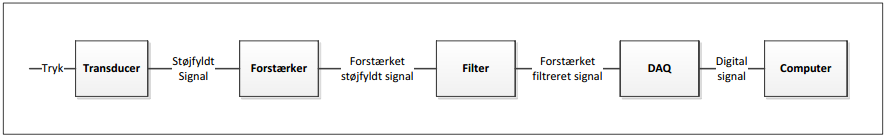
\includegraphics[scale=0.65]{so.PNG}
\caption{Blodtryksmålersystemet}
\end{figure}

Denne illustrerer, at der ind i transduceren kommer tryk og ud kommer et støjfyldt signal. Dette signal bliver ved forstærkeren forstærket og heraf et forstærket støjfyldt signal. Igennem filtret bliver støjen filtreret fra. Det filtrerede signal føres igennem DAQ’en, som omdanner det til et digitalt signal, som anvendes i computerens softwareprogram.\\
\newline
Til at præcisere komponenterne i blodtryksmålesystemets hardware, er der valgt at lave strukturdiagrammer. Her er der anvendt blokdefinitionsdiagram (BDD) og et internt blokdiagram (IBD).

\subsection{BDD}
BDD'et er anvendt til, at dokumentere nedbrydningen af systemet og forholdene mellem blokkene.  

\begin{figure}[H]
\centering
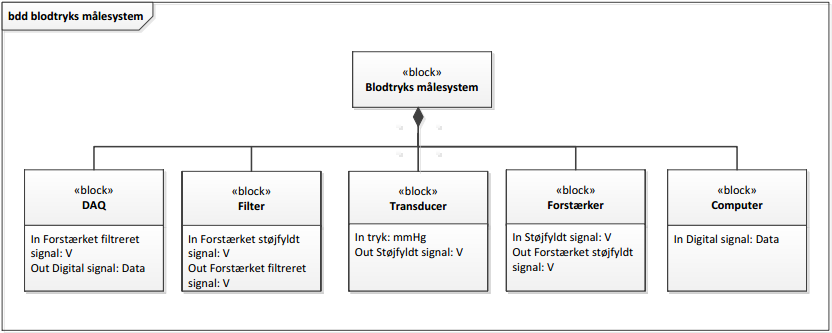
\includegraphics[scale=0.80]{bdd.PNG}
\caption{BDD}
\end{figure}

\textbf{Blokbeskrivelser:}
\begin{itemize}
\item Transducer: En tryktransducer, som konverterer et tryk til et analogt elektrisk signal
\item Forstærker: Signalet forstærkes således at hele forsyningsspændingen udnyttes
\item Filter: Et 2. ordens lavpasfilter fjerner højfrekvent støj
\item DAQ: A/D konverter omsætter den analoge indgangsspænding til et digitalt signal
\item Computer: Enheden som indeholder softwareprogrammet til visning af blodtryk
\end{itemize}
\subsection{IBD}
IBD'et er anvendt til, at dokumentere den interne struktur i blokkene.
\begin{figure}[H]
\centering
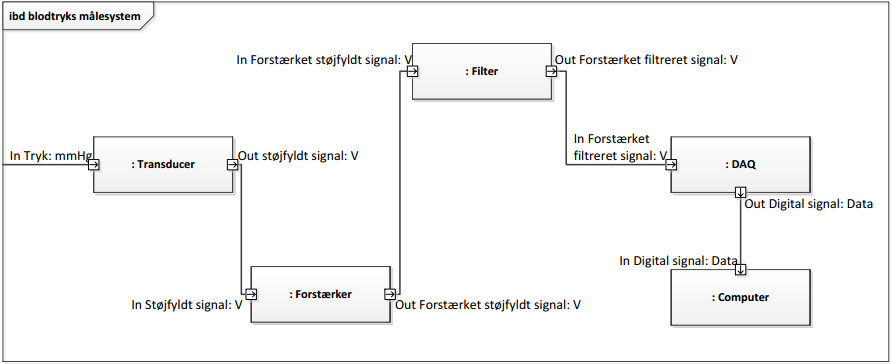
\includegraphics[scale=0.65]{ibd.PNG}
\caption{IBD}
\end{figure}




\subsubsection{Signalbeskrivelse}

\section{Software}
Brugergrænsefladen i software-delen består af to forskellige GUI'er, en til at logge ind og en til diagnostik. Programmet indeholder en række klasser indeholdende funktionaliteten beskrevet i UC's samt databaser til opbevaring af data. Softwaren er opbygget af trelagsmodellen. \\
\newline
For at skabe et overblik over sammenhængen mellem UC's og softwaren i systemet, er der udviklet en applikationsmodel. Applikationsmodellen indeholder en domænemodel over hele systemet, et klassediagram for hver enkelt UC, et sekvensdiagram over hele systemet, et sekvensdiagram for hver UC og et opdateret klassediagram med metoder. Ved at opdele de forskellige dele i softwaren samt at oprette klasser efter den ønskede funktionalitet i UC's, opnås en sammenhænge og overskuelighed over systemet som helhed.
\subsection{Domænemodel}
Domænemodellen er udviklet vha. navneordsanalyse i de fem UC's. Domænemodellen giver et overblik over hvilken funktionalitet der - ud fra UC's - er relevant. Funktionaliteterne er opdelt i kasser, der senere bliver til klasser i softwaren. 

\begin{figure}[H]
\centering
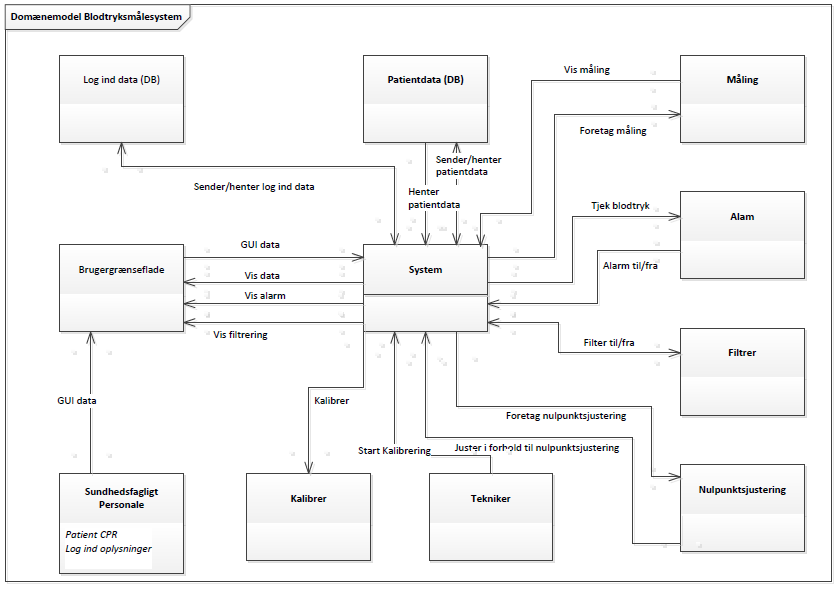
\includegraphics[scale=0.70]{dom.PNG}
\caption{Domænemodel blodtryksmålersystem}
\end{figure}

\subsection{Klassediagram}
Klassediagrammerne for hver enkelt UC viser sammenhængen mellem de forskellige instanser i den enkelte UC. \newline 
\textit{Boundary-klasser} er den akutuelle UC's aktører. \newline 
\textit{Controller-klassen} indeholder UC'ens funktionalitet og udfører UC'en ved at interagere med boundary-klasserne og domain-klasserne. Controller-klassen er opkaldt efter den aktuelle UC's navn. \newline
\textit{Domain-klassen} repræsenterer systemets domæne og hukommelse. 
%------------UC1----------------------------
\subsubsection{Klassediagram UC1}
I klassediagrammet for UC1 logger sundhedsfagligt personale ind vha. brugergrænsefladen - de er begge to boundary-klasser. Brugergrænsefladen sender besked til controller-klassen "Log ind". Log ind-data hentes, via controlleren, i Log ind databasen, og sendes tilbage til brugergrænsefladen via controlleren, hvorved sundhedsfagligt personale logges ind. 
%Metoder og attributter er opdateret efter konstruering af sekvensdiagram.
\begin{figure}[H]
\centering
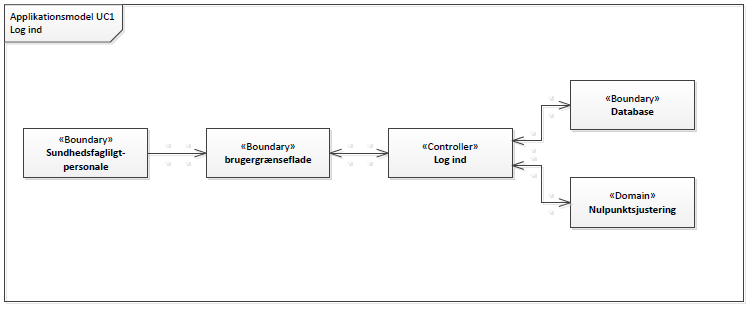
\includegraphics[scale=0.70]{app1.PNG}
\caption{Applikationsmodel UC1}
\end{figure}

%------------------UC2------------------------
\subsubsection{Applikationsmodel UC2}
I klassediagrammet for UC2 er sundhedsfagligt personale og brugergrænsefladen boundary-klasser. "Hent patientoplysninger" er UC'ens controller-klasse. Patientoplysningerne hentes fra Patient databasen - en boundary-klasse - og sendes tilbage igennem controller-klassen til brugergrænsefladen. 
\begin{figure}[H]
\centering
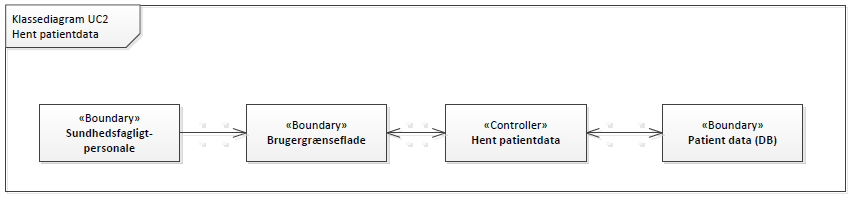
\includegraphics[scale=0.70]{app2.PNG}
\caption{Applikationsmodel UC2}
\end{figure}

%------------------UC3------------------------
\subsubsection{Applikationsmodel UC3}
I klassediagrammet for UC3 er sundhedsfagligt personale og brugergrænsefladen boundary-klasser. "Nulpunktsjuster"\ er UC'ens controller-klasse, som udfører UC'en vha. domain-klassen "Nulpunktsjustering". Nulpunktsjusteringen sendes tilbge til brugergrænsefladen fra domain-klassen, igennem controller-klassen.
\begin{figure}[H]
\centering
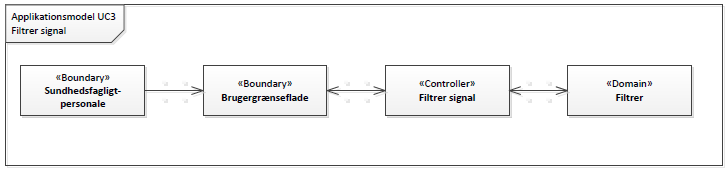
\includegraphics[scale=0.70]{app3.PNG}
\caption{Applikationsmodel UC3}
\end{figure}

%------------------UC4------------------------
\subsubsection{Applikationsmodel UC4}
Klassediagrammet for UC4 viser, at sundhedsfagligt personale og brugergrænsefladen er boundary-klasser. "Filtrer signal"\ er UC'ens controller-klasse som får besked fra brugergrænsefladen om at filtrere signalet - og sender filtreringen tilbage til brugergrænsefladen. 
\begin{figure}[H]
\centering
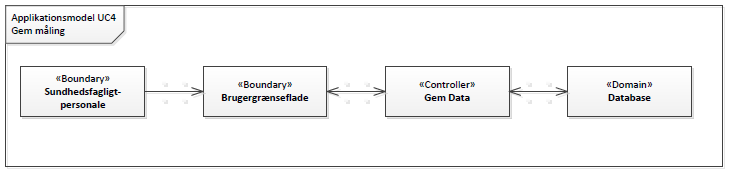
\includegraphics[scale=0.70]{app4.PNG}
\caption{Applikationsmodel UC4}
\end{figure}

%------------------UC5------------------------
\subsubsection{Applikationsmodel UC5}
I klassediagrammet for UC5 er sundhedsfagligt personale og brugergrænsefladen boundary-klasser. "Gem måling"\ er UC'ens controller-klasse, som får besked fra brugergrænsefladen om at gemme den akutelle måling. Denne information sendes videre til domain-klassen "Patientdata"\, som sender besked tilbage til brugergrænsefladen, igennem controller-klassen om, at data er gemt. 
\begin{figure}[H]
\centering
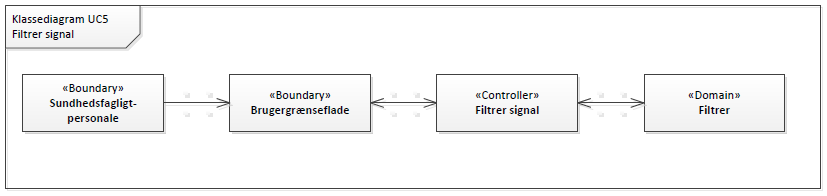
\includegraphics[scale=0.70]{app5.PNG}
\caption{Applikationsmodel UC5}
\end{figure}

%------------------UC6------------------------
\subsubsection{Applikationsmodel UC6}
I klassediagrammet for UC6 ses det, at tekniker og brugergrænsefladen er boundary-klasser. Teknikeren kalibrerer systemet i controller-klassen, som justerer brugergrænsefladen i forhold til kalibreringen. 
\begin{figure}[H]
\centering
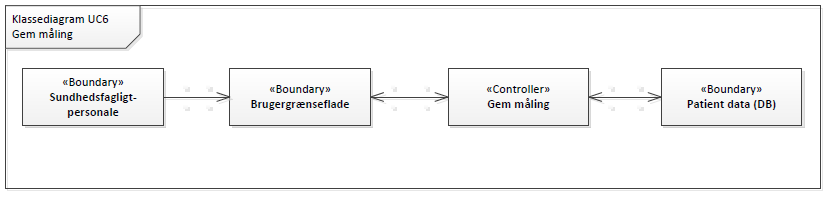
\includegraphics[scale=0.70]{app6.PNG}
\caption{Applikationsmodel UC6}
\end{figure}


